\documentclass{article}
\usepackage{graphicx}
\usepackage{tikz}

\begin{document}

\begin{figure}[h]
    \centering
    \begin{tikzpicture}
        % Replace 'UAV top view.jpeg' with your actual filename
        % If it still fails, try replacing the \node line with:
        % \draw (0,0) rectangle (5,3) node[midway]{Image Placeholder};
        
        \node[anchor=south west, inner sep=0] (image) at (0,0) {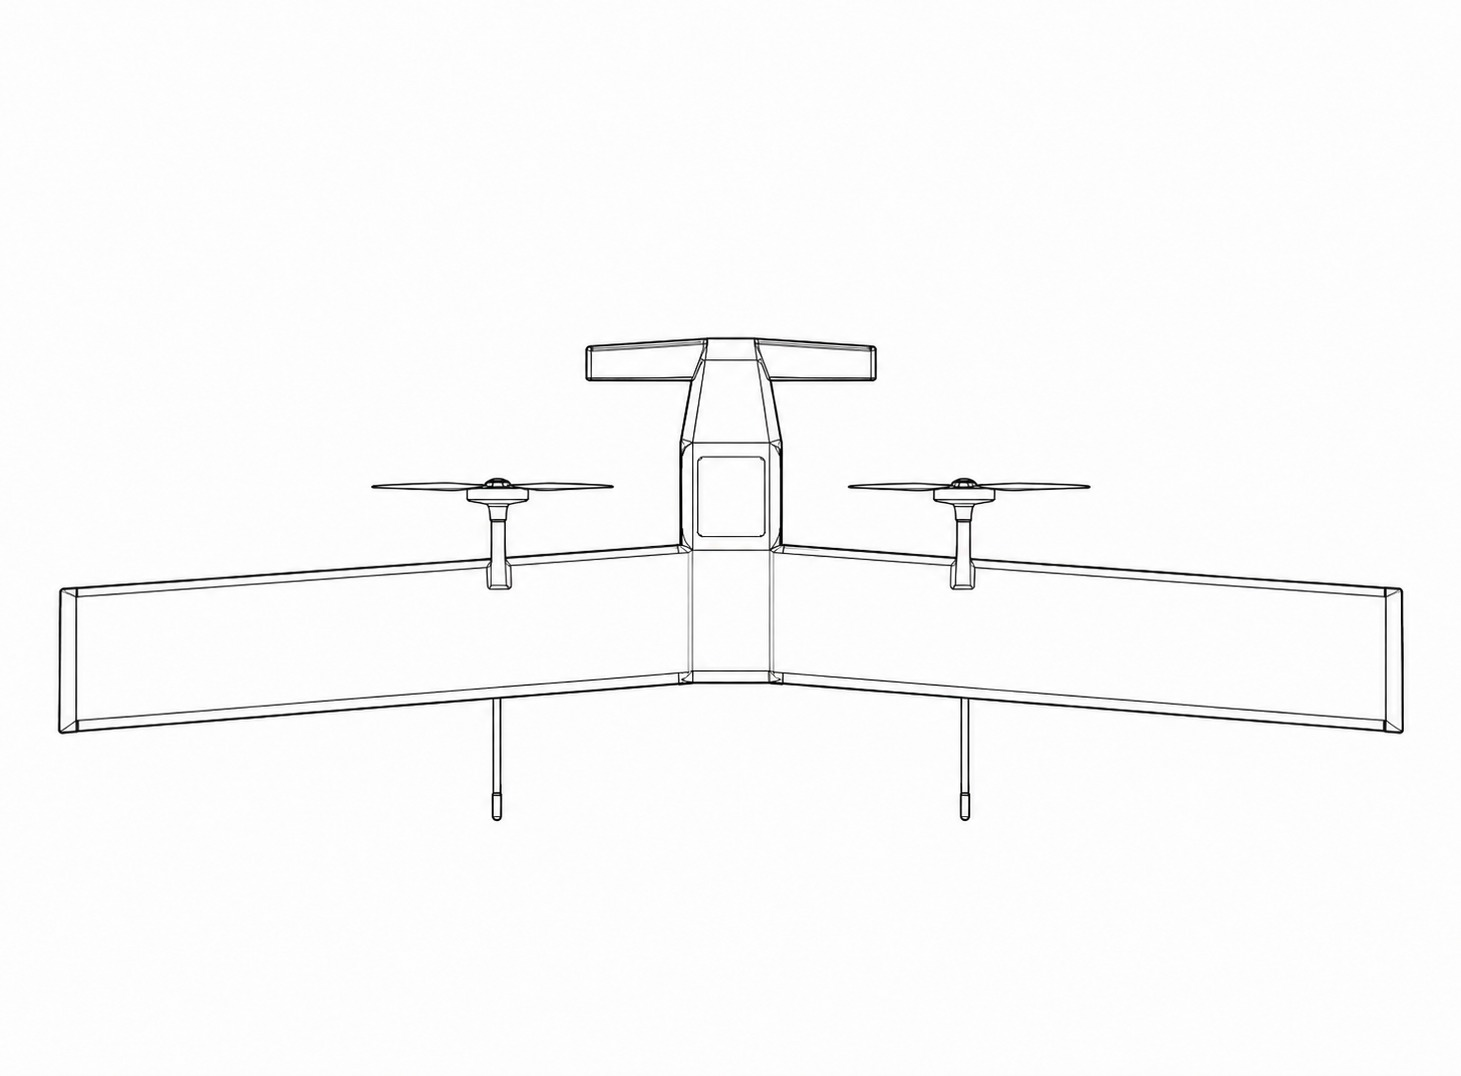
\includegraphics[width=0.8\textwidth]{UAV top view.jpeg}};

        \begin{scope}[x={(image.south east)},y={(image.north west)}]
            % Forces
            \coordinate (CG) at (0.5, 0.45);
            \draw[red, ultra thick, -stealth] (CG) -- ++(0, -0.15) node[below] {$W$};
            
            % Simple Grid to help you find coordinates (remove later)
            \draw[help lines, xstep=0.1, ystep=0.1] (0,0) grid (1,1);
        \end{scope}
    \end{tikzpicture}
    \caption{UAV Loading Diagram}
\end{figure}

\end{document}